%%%%%% DEPRECATED: Now it's a section on Masking chapter %%%%%%
\chapter{MaskD: Una Herramienta para medir masking-tolerancia a fallas}
\label{cap:maskD}

En este capítulo presentamos {\MaskD}, una herramienta automática diseñada para medir el nivel de tolerancia a fallas entre componentes de software, 
descritos por medio de un lenguaje de comandos con guardas.
La herramienta se enfoca en medir componentes masking-tolerantes a fallas, es decir, programas que enmascaran fallas de tal manera que no puedan ser observadas por el ambiente. Usualmente se lo clasifica como el el tipo de tolerancia mas beneficioso y es a su vez una propiedad altamente deseable para sistemas críticos. 
La herramienta toma como entrada un modelo nominal y un modelo de su implementación tolerante a fallas y computa automáticamente la distancia de masking entre ellos. 

La herramienta está diseñada para darle soporte a ingenieros de software para el análisis y diseño de sistemas tolerantes a fallas. Más precisamente, utiliza una función de distancia de masking de tal forma que el ingeniero pueda medir la masking-tolerancia de una implementación tolerante a fallas dada, i.e., la cantidad de fallas que la implementación es capaz de enmascarar en el peor caso posible. 
Por lo tanto, los ingenieros pueden medir y comparar la distancia de masking-tolerancia a fallas entre distintas implementaciones y el modelo nominal, y así seleccionar la implementación que mejor se adapte a sus preferencias.

\subsection{La Herramienta} \label{sec:mask_sec}

\MaskD~toma como entrada un modelo nominal y su implementación tolerante a fallas, y produce como salida la distancia de masking entre ellos, la cual es un valor en el intervalo $[0,1]$.
Los modelos de entrada se describen utilizando el lenguaje de comandos con guardas introducido en \cite{AroraGouda93}, un lenguaje de programación simple para describir algoritmos tolerantes a fallas.
Mas precisamente, un programa descrito en este lenguaje es una colección de procesos, donde cada proceso esta compuesto por una colección de acciones etiquetadas del estilo: $[Label]~Guard \rightarrow Command$, donde $Guard$ es una condición lógica sobre el estado actual del programa, $Command$ es una colección de asignaciones básicas que se ejecutan simultáneamente, y $Label$ es un nombre para la acción.
Estas construcciones sintácticas se denominan acciones. El lenguaje también permite a los usuarios etiquetar una acción como \emph{internal} (i.e., acciones silenciosas). Esto es importante para abstraerse de los mecanismos internos de el sistema que se modela y permitir construir modelos mas complejos. Además, algunas acciones pueden ser etiquetadas como \emph{faulty} para indicar que representan fallas. 

\begin{figure}[t]
\centering
\begin{minipage}[t]{.47\textwidth}
\fontsize{10}{10}\selectfont\ttfamily
\begin{tabbing}
x\=xxxxxxxx\=xxxxxxxxxxxx\=xx\=xxx\= \kill    
Process MEMORIA \{\\[1ex]
\>r : BOOL;  // valor observable \\ 
\>b0 : BOOL; // bit de memoria\\[1ex]
\>Initial: b0 \&\& r;\\[1ex]
%\>                   \>\>// 1 = refreshing\\[1ex]
\>[write1]  true -> b0=true, \\
\>\>~r=true; \\
\>[write0]  true -> b0=false, \\
\>\>~r=false; \\
\>[read0] !r -> r=r; // skip \\
\>[read1]  r -> r=r; // skip \\[1ex]
\}\\
\end{tabbing}
\end{minipage}
\caption{Modelo nominal para el ejemplo de la celda de memoria.} \label{fig:exam_1_mem_cell_nominal}
\end{figure}

\hfill

\begin{figure}[t]
\centering
\begin{minipage}[t]{.47\textwidth}
\fontsize{10}{10}\selectfont\ttfamily
\begin{tabbing}
x\=xxxxxxxx\=xxxxxxxxxxxxx\=xxx\=xxx\= \kill    
Process MEMORIA\_FT \{\\[1ex]
\>r : BOOL; // valor observable \\
\>b0 : BOOL; // primer bit \\
\>b1 : BOOL; // segundo bit \\
\>b2 : BOOL; // tercer bit \\[1ex]
%\>\textcolor{red}{f : [0..1] init 0;} \>\>\textcolor{red}{// fault limiting artifact}\\[1ex]
\>Initial: b0 \&\& b1 \&\& b2 \&\& r;\\[1ex]
\>[write1]  true -> b0=true, b1=true,  \\
\>\>~b3=true, r=true; \>\> \\
\>[write0]  true -> b0=false, b1=false,  \\
\>\>~b3=false, r=false; \>\> \\
\>[read0]  !r -> r=r; // skip \\
\>[read1]  r ->  r=r; // skip \\
\>[fault1]  faulty true -> b0=!b0, r =(!b0\&\&b1)||(b1\&\&b2)|| \\ 
\>\>(!b0\&\&b2); // el primer bit falla  \\
\>[fault2]  faulty true -> b1=!b1, r =(b0\&\&!b1)||(!b1\&\&b2)|| \\ 
\>\>(b0\&\&b2); // el segundo bit falla  \\
\>[fault3]  faulty true -> b2=!b2, r =(b0\&\&b1)||(b1\&\&!b2)|| \\ 
\>\>(b0\&\&!b2); // el tercer bit falla  \\[1ex]
\}\\
\end{tabbing}
\end{minipage}
\caption{Modelo con fallas para el ejemplo de la celda de memoria.} \label{fig:exam_1_mem_cell_faulty}
\end{figure}

Como ejemplo, consideremos la celda de memoria vista en el capitulo anterior. 
Un estado en este sistema mantiene el valor corriente de la celda de memoria ($m=i$, para $i=0,1$), la operación de escritura permite cambiar este valor, y la operación de lectura retorna el valor almacenado.  
En este sistema el resultado de una lectura dependerá del valor almacenado en la celda. 
Por lo tanto, una propiedad que uno podría asociar a este modelo es que el valor leído de la celda debe coincidir con el valor escrito por la ultima operación de escritura realizado por el sistema. 
    
Como se ha visto anteriormente, una falla potencial en este escenario ocurre cuando la celda pierde su carga de forma inesperada, y su valor almacenado cambia sin que se haya realizado una escritura (e.g., cambia de $1$ a $0$ por perdida de carga). Una técnica típica para lidiar con esta situación es el uso de \emph{redundancia}: 
en este caso, se utilizan tres bits de memoria en lugar de solo uno. Las operaciones de escritura son realizadas simultáneamente en los tres bits. 
La operación de lectura, por otro lado, retorna el valor que se repite al menos dos veces en los bits de memoria; esto se conoce como \emph{votación}. 
Las figuras \ref{fig:exam_1_mem_cell_nominal} y \ref{fig:exam_1_mem_cell_faulty} muestran los procesos representando el modelo nominal y el modelo de la implementación tolerante a fallas respectivamente para este ejemplo. 

\subsection{Arquitectura}

\MaskD~es software de código abierto escrito en el lenguaje \textsf{Java}. La documentación y las instrucciones de instalación se pueden encontrar en \cite{MaskD}. La arquitectura de la herramienta se muestra en la figura~\ref{fig:arch}.
\begin{figure}[t]
    \centering
    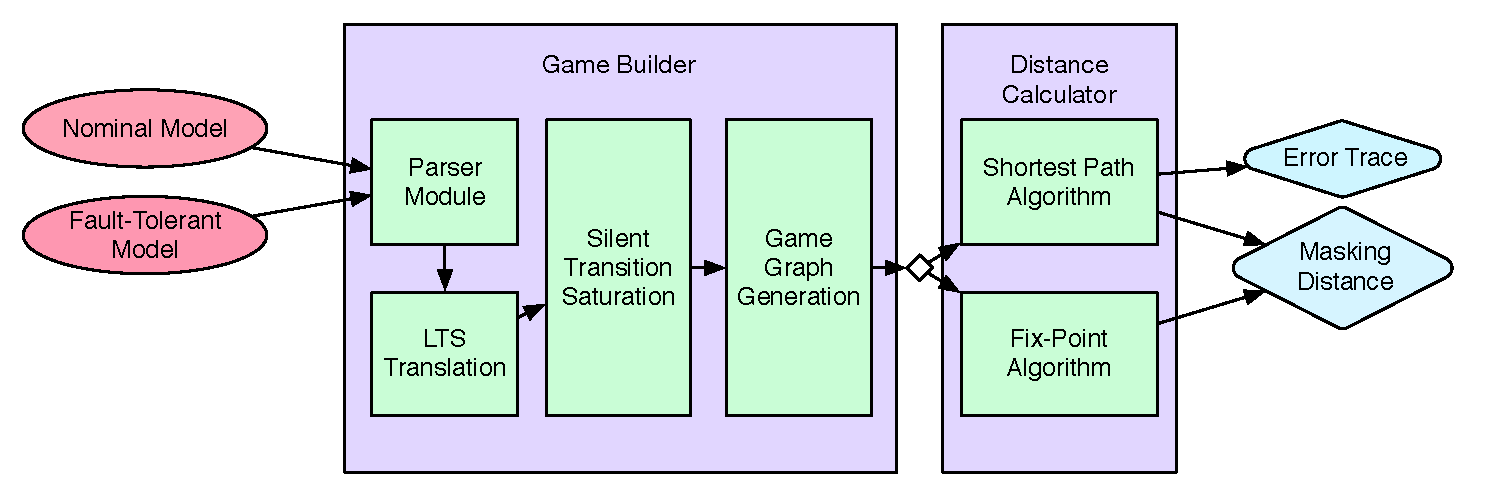
\includegraphics[scale=0.50]{Figs/architecture-eps-converted-to.pdf}
    \caption{Arquitectura de \textsf{MaskD}.}\label{fig:arch}
\end{figure}
    Discutiremos brevemente las componentes principales de la herramienta:
\begin{description}
    \item[Módulo Parser.] Realiza análisis sintáctico básico sobre los modelos de entrada y produce estructuras de datos que representan a  estas entradas. Para esto se utilizan las bibliotecas \textsf{Cup} y 
    \textsf{JFlex} para generar automáticamente el parser a partir de la gramática que describe el lenguaje de modelado.
    \item[Traducción a LTS.] Los modelos obtenidos del parser son traducidos a Sistemas de Transición Etiquetados (LTSs), i.e., 
    grafos donde los vértices representan estados del programa y donde las transiciones mantienen información sobre las acciones de los modelos. 
    \item[Saturación de Transiciones Silenciosas.] Las transiciones internas/silenciosas en los LTSs que representan los modelos de entrada son saturadas utilizando algoritmos estándar que provienen de teoría sobre álgebras de procesos \cite{Milner89}. Como resultado, se generan LTSs saturados, estos son necesarios para verificar la relación de masking cuando existen transiciones internas.
    \item[Generación del Grafo de Juego.] Utiliza los LTSs saturados para producir un grafo de juego. Los nodos en este grafo codifican la configuración corriente del juego: 
    el próximo jugador que debe jugar, la ultima acción jugada, y referencias a los estados de los LTSs de los modelos de entrada que se corresponden con la configuración actual del juego. 
    Las transiciones en este grafo corresponden a las posibles jugadas para los jugadores, i.e.,  transiciones en los LTSs originales.
    \item[Algoritmo de Camino mas Corto.] Si los modelos de entrada son deterministas en las etiquetas de sus acciones, el algoritmo de camino mas corto de Dial es utilizado para obtener el camino mas corto hacia el estado de error, desde el cual se calcula el valor final.
    \item[Algoritmo de Punto Fijo.] Este es el algoritmo por defecto, funciona tanto para modelos deterministas como no deterministas en las etiquetas de sus acciones, utiliza una búsqueda de estilo bottom-up breadth-first para computar el valor del juego. 
    Este algoritmo se basa en algoritmos conocidos para resolver juegos de alcanzabilidad que utilizan conjuntos \emph{atractores} \cite{Jurd11}. 
    %This algorithm is polynomial in the game graph size.
\end{description}
Como se ha explicado mas arriba, un punto interesante sobre la herramienta es que, para sistemas deterministas en sus acciones, la distancia de masking entre dos sistemas puede ser computada recurriendo al algoritmo de camino mas corto de Dial \cite{Dial69}, el cual tiene complejidad lineal con respecto al tamaño de los grafos utilizados para representar los sistemas.
En el caso de los sistemas no deterministas, se necesita un recorrido del estilo 
breadth-first con punto fijo, lo cual hace que el algoritmo sea menos eficiente. Sin embargo, aun en este caso sigue siendo polinomial. 

%TODO: draw architecture and explain

%In order to measure the degree of masking fault-tolerance of a given system, 
%we start characterizing masking fault-tolerance via simulation relations between 
%two systems as defined in \cite{DemasiCMA17}. 
%The first one acting as a specification 
%of the intended behavior (i.e., nominal model) and the 
%second one as the fault-tolerant implementation (i.e., the extended model with 
%faulty behavior).
%The existence of a masking relation implies that the implementation masks the faults.
%Afterwards, we introduce a game characterization of 
%masking simulation and we enrich the resulting games 
%with quantitative objectives to define the notion of 
%\emph{masking fault-tolerance distance}, 
%where the possible values of the game belong to the interval $[0,1]$. 

\subsection{Modo de Uso}

El comando estándar para ejecutar {\MaskD} en un sistema operativo de estilo Unix es:
\\ 
\\
 \verb"./MaskD <options> <spec_path> <imp_path>"
\\
\\
En este caso la herramienta arroja como resultado la distancia de masking entre la especificación y la implementación utilizando el algoritmo por defecto (algoritmo de punto fijo).
Algunos comandos opcionales incluyen: \verb"-t: print error trace", el cual muestra por salida estándar una traza hasta el estado de error bajo estrategias óptimas; y  \verb"-s: start simulation", el cual comienza una simulación manual desde el estado inicial.  
Obtener un camino hacia el estado de error es una funcionalidad útil para encontrar defectos en las descripciones de programas, los cuales pueden fallar por razones no intencionales. A su vez la traza sirve para ver como se comportan las estrategias óptimas de los jugadores. Una traza para el ejemplo de la celda de memoria se muestra en la figura~\ref{fig:trace_mem_cell}. Los estados se muestran en el formato \verb"{spec_state, last_action_played, imp_state, player_turn}", donde \verb"spec_state" es el estado corriente del modelo nominal, \verb"last_action_played" es la última acción que se jugó (solo es relevante para estados del Verificador), \verb"imp_state" es el estado del modelo que representa a la implementación y \verb"player_turn" es el jugador cuyo turno corresponde jugar. En este caso, después de dos fallas (bits que cambian de valor sin que haya una escritura), al luego realizar una lectura, nos lleva al estado de error ya que en el modelo nominal el valor de la celda es $0$, mientras que el el modelo tolerante a fallas el valor leído en la mayoría (votación) de bits es $1$. Por otro lado, la funcionalidad de simulación permite al usuario seleccionar manualmente las acciones disponibles en cada punto del juego de masking, lo cual también es útil para verificar que los modelos se comportan como el usuario espera.
Por defecto, \MaskD~computa la distancia de masking para una entrada dada utilizando el algoritmo para sistemas no deterministas. 
El usuario puede utilizar la opción \verb"-det" para cambiar al algoritmo de distancia de masking para sistemas deterministas.
\begin{figure}[t]
\centering
\begin{minipage}[t]{.47\textwidth}
\fontsize{10}{10}\selectfont\ttfamily
\begin{tabbing}
0. \{ <mr,mb0> , \# , <mr,mb0,mb1,mb2> , R \} \\ 
1. \{ <mr,mb0> , I\_m.fault1 , <mr,mb1,mb2> , V \} \\ 
2. \{ <mr,mb0> , \# , <mr,mb1,mb2> , R \} \\ 
3. \{ <mr,mb0> , I\_m.fault2 , <mb2> , V \} \\ 
4. \{ <mr,mb0> , \# , <mb2> , R \} \\ 
5. \{ <mr,mb0> , S\_m.read1 , <mb2> , V \} \\ 
6. ERR\_STATE \\ 
\end{tabbing}
\end{minipage}
\caption{Traza de Error para el ejemplo de la celda de memoria.} \label{fig:trace_mem_cell}
\end{figure}






